\setscratch{scale=0.85}

\themaG
\graphicspath{{../Ch13_Se_deplacer_sur_un_plan/Images/}}

\chapter{Se déplacer}
\label{C18}


%%%%%%%%%%%%%%%%%%%%%%%%%%%%%%%%%%%%%%
\begin{prerequis}[Connaissances et compétences abordées]
   \begin{itemize}
      \item Décrire ou exécuter des déplacements, sur un plan ou sur une carte (école, quartier, ville, village).
      \item Accomplir, décrire, coder des déplacements dans des espaces familiers.
      \item Programmer les déplacements d’un robot ou ceux d’un personnage sur un écran en utilisant un logiciel de programmation.
      \item Vocabulaire permettant de définir des positions et des déplacements (tourner à gauche, à droite ; faire demi-tour, effectuer un quart de tour à droite, à gauche).
   \end{itemize}
\end{prerequis}

\vfill

\begin{debat}[Débat : les douze travaux d'Hercule] 
   Les 12 travaux d'Hercule sont les exploits exécutés par Hercule sur l'ordre d'Eurysthée. Ils constituent l'un des épisodes les plus célèbres de la mythologie grecque. Les 12 travaux sont les suivants :
   \begin{itemize}
      \item Étouffer le lion de Némée à la peau impénétrable, et rapporter sa dépouille.
      \item Tuer l'hydre de Lerne, dont les têtes tranchées repoussaient sans cesse.
      \item Ramener vivant l'énorme sanglier d'Érymanthe.
      \item Capturer la biche de Cérynie aux sabots d'airain et aux bois d'or, créature sacrée d'Artémis.
      \item Tuer les oiseaux du lac Stymphale aux plumes d'airain.
      \item Nettoyer les écuries d'Augias, si grandes que personne n'avait jamais eu le courage de le faire.
      \item Dompter le taureau crétois de Minos, que celui-ci n'avait pas voulu sacrifier à Poséidon.
      \item Capturer les cavales de Diomède (juments mangeuses d'hommes).
      \item Rapporter la ceinture d'Hippolyte, fille d'Arès et reine des Amazones.
      \item Vaincre le géant aux trois corps Géryon, et voler son troupeau de bœufs.
      \item Descendre aux Enfers et enchaîner Cerbère, le chien aux trois têtes puis le présenter à Eurysthée.
      \item Rapporter les pommes d'or du jardin des Hespérides, que gardait Ladon.
   \end{itemize}
   \begin{center} 
      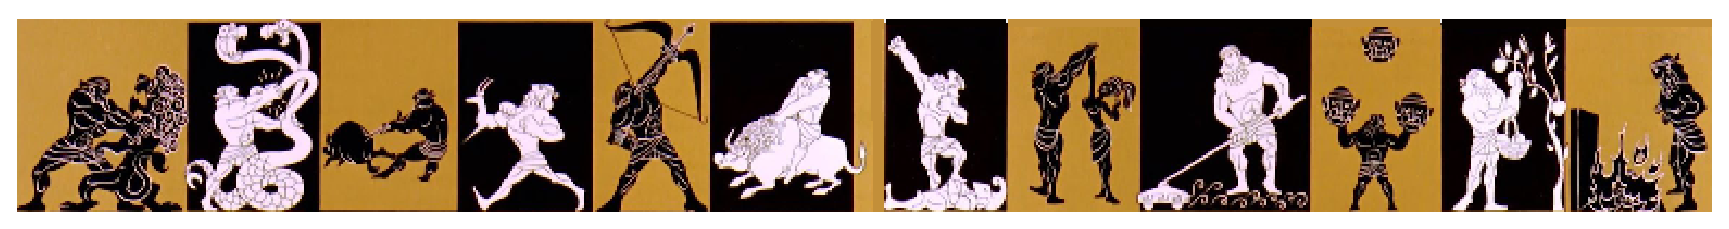
\includegraphics[width=11cm]{travaux}
   \end{center}
   \begin{cadre}[B2][F4]
      \begin{center}
         Vidéo : \href{https://www.youtube.com/watch?v=NWgaJvStk6U}{\bf L'invincible Hercule et ses douze travaux} de Laurent Bègue aux éditions {\it Belize}.
      \end{center}
   \end{cadre}
\end{debat}

\vfill

\textcolor{PartieGeometrie}{\sffamily\bfseries Cahier de compétences} : 26 p. 80 ; 43 p. 109.


%%%%%%%%%%%%%%%%%%%%%%%%%%%%%
%%%%%%%%%%%%%%%%%%%%%%%%%%%%%
\activites

\begin{activite}[Un robot nommé Hercule]
   {\bf Objectifs :} se repérer, décrire et exécuter des déplacements sur un plan.
   \begin{QCM}
      \partie[lecture du texte n\degre3 des 12 travaux d'Hercule. Capturer le sanglier d'Erymanthe]
         \ \\
         \hspace*{1cm}
         \begin{minipage}{14CM}
            Le sanglier d’Erymanthe était une bête sauvage que personne n’osait approcher et qui faisait d’énormes ravages dans les cultures des paysans. Ramener ce sanglier vivant était une épreuve impossible pour un être humain, mais pas pour un demi-dieu\dots \\
            
            Les paysans du mont Erymanthe implorèrent Eurysthée de faire quelque chose contre l’énorme sanglier qui dévastait leurs cultures, dévorait leurs troupeaux et anéantissait leurs récoltes. Eurysthée ordonna à Hercule de capturer ce sanglier et de le lui amener vivant. Il espérait rendre ainsi Hercule ridicule aux yeux du peuple qui l’admirait un peu trop au goût du souverain. \\
            
            Il fallut plusieurs jours à Hercule pour rejoindre la rivière Erymanthe. Il en remonta le cours jusqu’au sommet de la montagne où les paysans s’agenouillèrent devant Hercule en l’implorant de les délivrer de ce monstre qui ravage leurs cultures. Il fut facile pour Hercule de pister le sanglier car il était si lourd que ses traces étaient fortement marquées sur le sol. De plus les arbres étaient lacérés et la terre retournée partout où la bête était passée. \\
            
             Il finit par se trouver nez à nez avec l’animal. Mais ne pouvant utiliser ses armes de peur de blesser ou de tuer l’animal, Hercule le vit s’enfuir. Il passa ensuite plusieurs jours à explorer le mont Erymanthe et à étudier les habitudes du sanglier. Après plusieurs tentatives infructueuses pour le capturer, Hercule changea sa stratégie. Il passa plusieurs semaines à creuser des fossés, bouger des pierres, créer des impasses et encore agrandir des sentiers sur le mont Erymanthe. \\
             
            Un matin d’hiver, la neige se mit à tomber recouvrant le mont. Hercule repéra aisément les traces du sanglier dans la neige et se mit à le poursuivre. À la fin de la journée, comme Hercule l’espérait, le sanglier s’engagea sur un sentier qu’il avait modifié débouchant sur un petit ravin. Le sanglier ne pouvait plus lui échapper. \\
            
            \begin{minipage}{8cm}
               La bête tomba dans le ravin mais sa chute fut amortie par la neige. Il fut juste assommé. Hercule n’eut plus qu’à ficeler les pattes de l’animal et à le hisser sur son dos afin de l’amener à son cousin Eurysthée.
            \end{minipage}
            \qquad
            \begin{minipage}{5cm}
               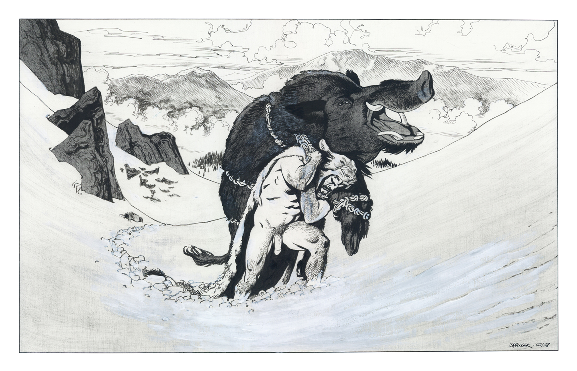
\includegraphics[width=5cm]{capture_sanglier} \\ [2mm]
            \end{minipage}
         \end{minipage}
   \end{QCM}

\hfill{\footnotesize {https://www.les-12-travaux-hercule.fr/les-12-travaux/le-sanglier-derymanthe/}}

\pagebreak

\begin{landscape}

Prénom : \pf \\ [1cm]

\begin{minipage}{2cm}
   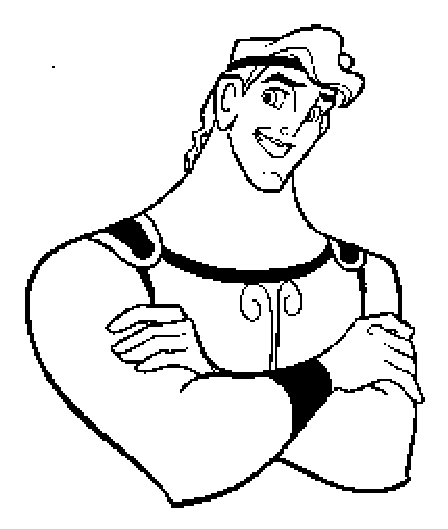
\includegraphics[width=1.7cm]{Hercule}
\end{minipage}
\begin{minipage}{19cm}
\begin{center}
{\huge Un robot nommé Hercule} \\ [5mm]
    Imagine un code (des signes) permettant de créer un programme pour déplacer Hercule vers le sanglier d’Erymanthe.
\end{center}
\end{minipage}
\begin{minipage}{3cm}
   \includegraphics[width=2.8cm]{Sanglier}
\end{minipage}

\medskip

\begin{tabular}{|p{1.8cm}|*{5}{p{3.8cm}|}}
   \hline
   Instruction & & & & & \\
   \hline
   \vspace*{0.7cm}
   Code \newline
   \vspace*{1cm}
   & & & & & \\
   \hline
\end{tabular}

\bigskip

\begin{center}
    Le code retenu collectivement.
\end{center}

\begin{tabular}{|p{1.8cm}|*{5}{C{3.8}|}}
   \hline
   Instruction & & & & & \\
   \hline
   \vspace*{0.7cm}
   Code \newline
   \vspace*{1cm}
   & & & & & \\
   \hline
\end{tabular}

\end{landscape}

\end{activite}


%%%%%%%%%%%%%%%%%%%%%%%%%%%%%%%%%%
%%%%%%%%%%%%%%%%%%%%%%%%%%%%%%%%%%
\cours 

%%%%%%%%%%%%%%%%%%%%%%%%%%%%%%%%%
\section{Se déplacer}
 
\begin{methode}[Langages de déplacement]
   Pour se déplacer dans le plan, il existe principalement deux langages de déplacement :
   \begin{itemize}
      \item le langage {\bf absolu} composé des mots de vocabulaire du type : \og haut \fg{}, \og bas \fg{}, \og droite \fg{} et \og gauche \fg. Le déplacement se fait comme si on se plaçait en vue du dessus ;
      \item le langage {\bf relatif} composé des mots de vocabulaire du type : \og avancer \fg{}, \og tourner à droite \fg{} et \og tourner à gauche \fg. C'est ici le point de vue de l'observateur qui est adopté.
   \end{itemize}
   \exercice
   \begin{center}
   \psset{unit=0.7}
   \begin{pspicture}(0,-1)(5,4)
      \psgrid[subgriddiv=1,gridlabels=0mm](0,-1)(5,4)
      \psset{linecolor=A1,arrowsize=3mm,linewidth=0.5mm}
      \psdots(0.5,0.5)(3.5,2.5)     
      \psline{->}(0.5,0.5)(2.5,0.5)(2.5,2.5)(3.5,2.5)
   \end{pspicture}
   \end{center}
   \correction
   \begin{minipage}{4cm}
      Avec le langage absolu : \\
      \og droite \\
      droite \\
      haut \\
      haut \\
      droite \fg
   \end{minipage}
   \qquad
   \begin{minipage}{4cm}   
     Avec le langage relatif : \\
     \og avancer \\
     avancer \\
     tourner à gauche \\
     avancer \\
     avancer \\
     tourner à droite \\
     avancer \fg
   \end{minipage}
\end{methode}


%%%%%%%%%%%%%%%%%%
\section{Codage et programmation}

\begin{definition}
   Un {\bf algorithme} est une liste ordonnée d'instructions permettant
de réaliser une tâche de manière automatisée.
\end{definition}

\bigskip

Un algorithme peut être traduit grâce à un langage de programmation. Au collège, on utilise {\bf Scratch}.

\begin{center}
   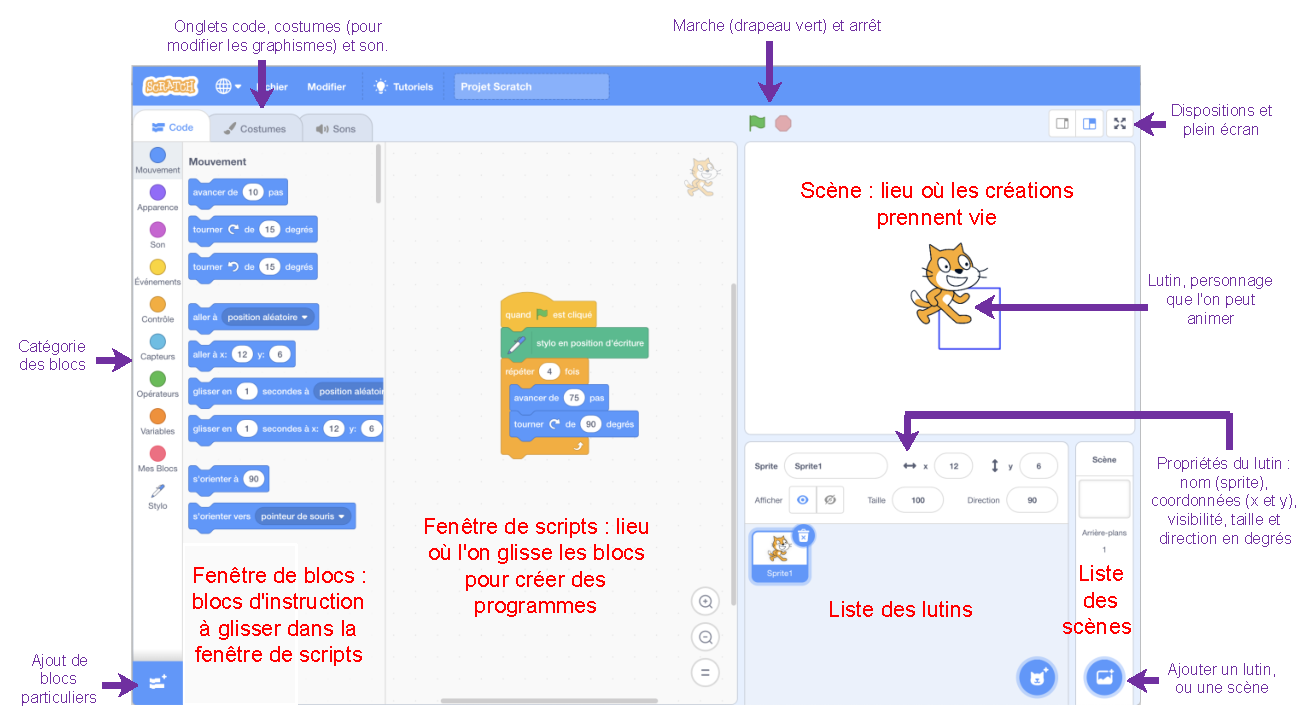
\includegraphics[width=16cm]{Scratch_interface}
\end{center}

\vspace*{-10mm}


%%%%%%%%%%%%%%%%%%%%%%%%%%%%%%%%%%%%%
\exercicesbase

\serie{Se déplacer}

\begin{exercice} %1
   \psset{unit=0.8}
   On dispose des instructions suivantes : \fbox{N} \; $\uparrow$ \; \fbox{S} \; $\downarrow$ \; \fbox{E} \; $\rightarrow$ \; \fbox{O} \; $\leftarrow$. \\
   Par exemple, la séquence NEESO donne \begin{pspicture}(-0.2,0)(2,1.5) \psline(0,0)(0,1)(2,1)(2,0)(1,0) \end{pspicture}
   \begin{enumerate}
      \item Écrire une séquence d'instructions permettant de tracer chacune des frises suivantes :
      \begin{colenumerate}{2}
         \item
         \begin{pspicture}(0,0.3)(8,1.5)
            \psline(0,1)(0,0)(1,0)(1,1)(2,1)(2,1)(2,0)(3,0)(3,1)(4,1)(4,1)(4,0)(5,0)(5,1)(6,1)(6,1)(6,0)(7,0)(7,1)(8,1)
         \end{pspicture} \\
         \item
         \begin{pspicture}(0,0.3)(8,1.5)
            \psline(0,0)(1,0)(1,1)(2,1)(2,0)(4,0)(4,1)(5,1)(5,0)(7,0)(7,1)(8,1)(8,0)(9,0)
         \end{pspicture} \\
         \item
         \begin{pspicture}(0,1.5)(8,2.5)
            \psline(0,1)(0,0)(1,0)(1,2)(2,2)(2,0)(3,0)(3,2)(4,2)(4,0)(5,0)(5,2)(6,2)(6,0)(7,0)(7,2)(8,2)(8,1)
         \end{pspicture}
      \end{colenumerate}
      \item Quand on répète une séquence d'instructions plusieurs fois, on peut utiliser une boucle \og répéter \fg. Effectuer le tracé correspondant aux séquences suivantes :
      \begin{colenumerate}{3}
         \item \texttt{répéter \fbox{4} fois} \\
         \hspace*{5mm} \psline(0,-0.2)(0,0.5) \; ENE
         \item \texttt{répéter \fbox{2} fois} \\
         \hspace*{5mm} \psline(0,-0.2)(0,0.5) \; NESSENE
         \item \texttt{répéter \fbox{3} fois} \\
         \hspace*{5mm} \psline(0,-0.2)(0,0.5) \; NNEESON
      \end{colenumerate}
      \smallskip
      \item Pour chaque frise de la question 1), écrire un programme optimisé en utilisant une boucle \og Répéter \fg.
   \end{enumerate}
\end{exercice}

\medskip

\begin{exercice} %2
   Un programme permet à un robot de se déplacer sur les cases d'un quadrillage. Chaque case atteinte est colorée en gris. Au début d'un programme, toutes les cases sont blanches, le robot se positionne sur une case de départ indiquée par un \og {\bf d} \fg{} et la colore aussitôt en gris. \\
Le robot se déplace suivant un programme grâce à un langage absolu dont le vocabulaire est
   \begin{center}
      \og S (south) ; E (east) ; N (north) ; W (west) \fg.
   \end{center}
   Voici des exemples de programmes et leurs effets :
   \begin{center}
   \begin{tabular}{|p{1.5cm}|C{2.5}|C{2.7}||p{1.5cm}|C{2.5}|C{2.7}|}
      \hline
      1W
      &
      Le robot avance de 1 case vers l'ouest.
      &
      \psset{unit=0.5cm}
      \begin{pspicture}(1,2)(3,3.5)
         \psframe[fillstyle=solid,fillcolor=lightgray](1,1)(3,2)
         \psgrid[gridlabels=0,subgriddiv=1,gridcolor=gray](0,0)(4,3)
         \rput(2.5,1.5){\textbf{d}}
      \end{pspicture}
      &
      2E 1W 2N
      &
      Le robot avance de 2 cases vers l'est, puis de 1 case vers l'ouest,
puis de 2 cases vers le nord.
      &
      \psset{unit=0.5cm}
      \begin{pspicture}(0,4.4)(5,6)
         \pspolygon[fillstyle=solid,fillcolor=lightgray](1,1)(4,1)(4,2)(3,2)(3,4)(2,4)(2,2)(1,2)
         \psgrid[gridlabels=0,subgriddiv=1,gridcolor=gray](5,5)
         \rput(1.5,1.5){\textbf{d}}
      \end{pspicture} \\
      \hline
   \end{tabular}
   \end{center}
   \begin{enumerate}
      \item Voici un programme : {\bf 1W 2N 2E 4S 2W} \\
      On souhaite dessiner le motif obtenu avec ce programme. Sur votre copie, réaliser ce motif en utilisant des carreaux, comme dans les exemples précédents. On marquera un \og \textbf{d} \fg{} sur la case de départ.
      \item On fait fonctionner un programme qui dessine le motif suivant :
      \psset{unit=0.5cm}
      \begin{pspicture}(-2,0)(8,3.5)
         \pspolygon[fillstyle=solid,fillcolor=lightgray](0,2)(1,2)(1,1)(2,1)(2,2)(3,2)(3,1)(4,1)(4,2)(5,2)(5,1)(6,1)(6,2)(7,2)(7,0)(0,0)
         \psgrid[gridlabels=0,subgriddiv=1,gridcolor=gray](-1,-1)(8,3)
         \rput(0.5,1.5){\textbf{d}}
      \end{pspicture} \begin{enumerate}
         \item Proposer un programme permettant de dessiner ce motif.
         \item Comment pourrait-on faire évoluer l'écriture de ce programme afin qu'il soit plus compact ?
      \end{enumerate}
   \end{enumerate}
\end{exercice}

\hfill{\footnotesize\it Source : inspiré du DNB 2019, Asie.}
   
\serie{La fourmi de Langton}

La fourmi de Langton\footnote{du nom de son inventeur le scientifique américain Christopher Langton. Ce système a été inventé vers la fin des années 1980.} est un automate qui se déplace dans un quadrillage suivant les règles suivantes :
\begin{itemize}
   \item au départ, toutes les cases sont de la même couleur, ici blanches ;
   \item si la fourmi est sur une case blanche, elle tourne de 90\degre{} vers la droite, change la couleur de la case en noir et avance d'une case ;
   \item si la fourmi est sur une case noire, elle tourne de 90\degre{} vers la gauche, change la couleur de la case en blanc et avance d'une case.
\end{itemize}

Compléter dans les quadrillages ci-dessous les 15 premières étapes du déplacement de la fourni. \\
Quelques étapes intermédiaires sont données afin de pouvoir vérifier que l'algorithme est correctement suivi.

\begin{center}
\psset{unit=0.5,subgriddiv=1,gridlabels=0mm,gridcolor=gray}
\small
\newcommand{\fourmi}[3]{\rput{#3}(#1,#2){\psdot[linecolor=red,dotstyle=triangle*,linewidth=1mm](0,0)}}
\begin{pspicture}(0,-0.7)(7,7)
   \psgrid(0,0)(7,7)
   \fourmi{3.5}{3.5}{0}
   \rput(3.5,-0.5){étape 0}
\end{pspicture}
\quad
\begin{pspicture}(0,-0.7)(7,7)
   \psframe[fillstyle=solid,fillcolor=darkgray](3,3)(4,4)
   \psgrid(0,0)(7,7)
   \fourmi{4.5}{3.5}{-90}
   \rput(3.5,-0.5){étape 1}
\end{pspicture}
\quad
\begin{pspicture}(0,-0.7)(7,7)  
   \psframe[fillstyle=solid,fillcolor=darkgray](3,3)(5,4)
   \psgrid(0,0)(7,7)
   \fourmi{4.5}{2.5}{180}
   \rput(3.5,-0.5){étape 2}
\end{pspicture}
\quad
\begin{pspicture}(0,-0.7)(7,7)
   \psgrid(0,0)(7,7)
   \rput(3.5,-0.5){étape 3}
\end{pspicture}

\bigskip

\begin{pspicture}(0,-0.7)(7,7)
   \psframe[fillstyle=solid,fillcolor=darkgray](3,2)(5,4)
   \psgrid(0,0)(7,7)
   \fourmi{3.5}{3.5}{0}
   \rput(3.5,-0.5){étape 4}
\end{pspicture}
\quad
\begin{pspicture}(0,-0.7)(7,7)
   \psgrid(0,0)(7,7)
   \rput(3.5,-0.5){étape 5}
\end{pspicture}
\quad
\begin{pspicture}(0,-0.7)(7,7)
   \psgrid(0,0)(7,7)
   \rput(3.5,-0.5){étape 6}
\end{pspicture}
\quad
\begin{pspicture}(0,-0.7)(7,7)
   \psframe[fillstyle=solid,fillcolor=darkgray](2,3)(3,5)
   \pspolygon[fillstyle=solid,fillcolor=darkgray](3,2)(5,2)(5,4)(4,4)(4,3)(3,3)
   \psgrid(0,0)(7,7)
   \fourmi{3.5}{4.5}{-90}
   \rput(3.5,-0.5){étape 7}
\end{pspicture}

\bigskip

\begin{pspicture}(0,-0.7)(7,7)
   \psgrid(0,0)(7,7)
   \rput(3.5,-0.5){étape 8}
\end{pspicture}
\quad
\begin{pspicture}(0,-0.7)(7,7)
   \psgrid(0,0)(7,7)
   \rput(3.5,-0.5){étape 9}
\end{pspicture}
\quad
\begin{pspicture}(0,-0.7)(7,7)
   \psgrid(0,0)(7,7)
   \rput(3.5,-0.5){étape 10}
\end{pspicture}
\quad
\begin{pspicture}(0,-0.7)(7,7)
   \pspolygon[fillstyle=solid,fillcolor=darkgray](2,2)(5,2)(5,4)(4,4)(4,5)(2,5)(2,4)(3,4)(3,3)(2,3)
   \psgrid(0,0)(7,7)
   \rput(3.5,-0.5){étape 11}
   \fourmi{1.5}{2.5}{90}
\end{pspicture}

\bigskip

\begin{pspicture}(0,0)(7,7)
   \psgrid(0,0)(7,7)
   \rput(3.5,-0.5){étape 12}
\end{pspicture}
\quad
\begin{pspicture}(0,0)(7,7)
   \psgrid(0,0)(7,7)
   \rput(3.5,-0.5){étape 13}
\end{pspicture}
\quad
\begin{pspicture}(0,0)(7,7)
   \psgrid(0,0)(7,7)
   \rput(3.5,-0.5){étape 14}
\end{pspicture}
\quad
\begin{pspicture}(0,0)(7,7)
   \psgrid(0,0)(7,7)
   \rput(3.5,-0.5){étape 15}
\end{pspicture} 
\end{center}


%%%%%%%%%%%%%%%%%%%%%%%%%%%%%%%%%%%%%
%%%%%%%%%%%%%%%%%%%%%%%%%%%%%%%%%%%%%
\Recreation

\enigme[Créer un jeu avec Scratch]
   \partie[présentation du jeu]
      L'objectif est de créer un jeu dans lequel un lutin (le chasseur) doit attraper d'autres lutins (les proies). \\
      Les programmes pour cette première découverte de Scratch vous seront tous donnés, nous discuterons de la manière dont ils ont été constitués une fois que vous les aurez testés !
      \begin{center}
         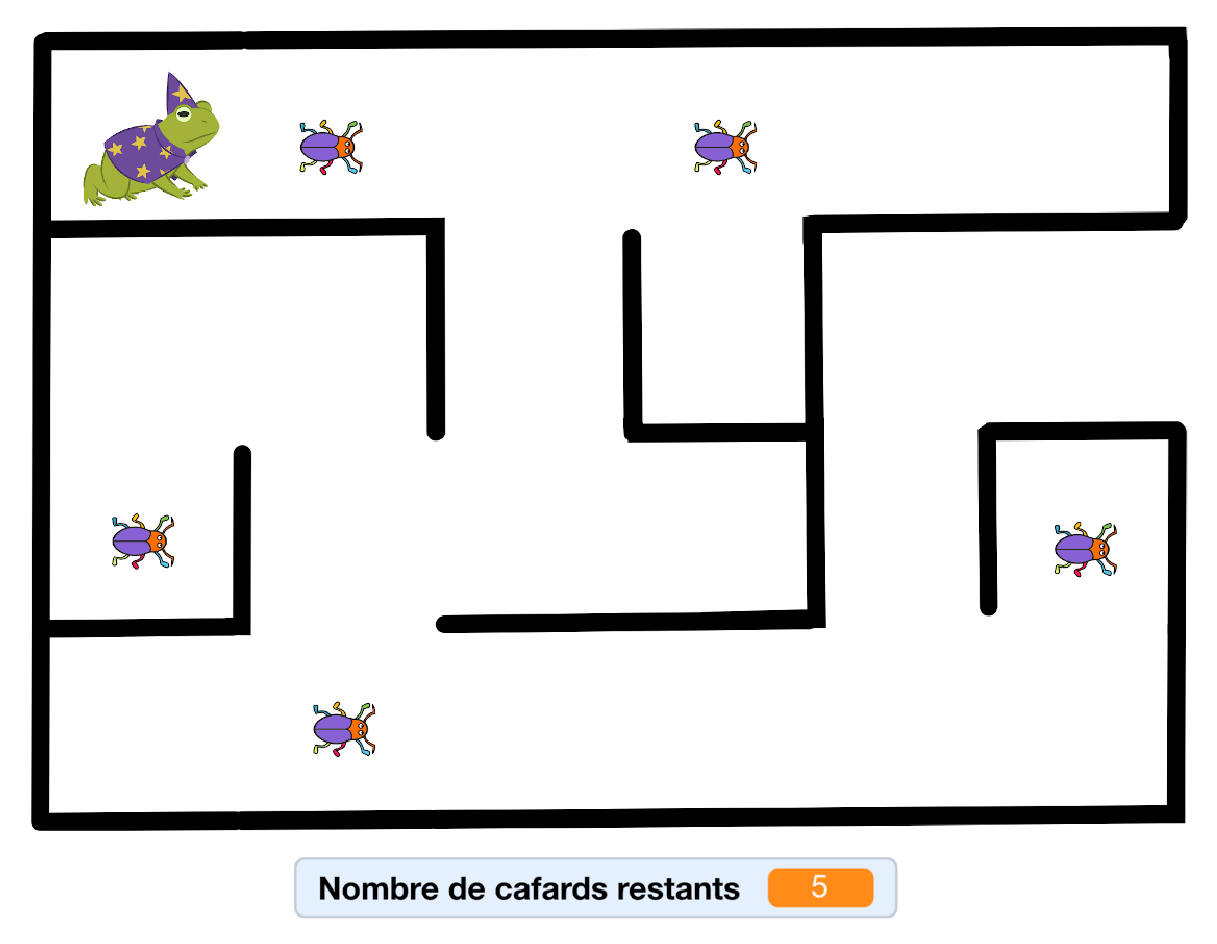
\includegraphics[width=10cm]{Scratch_jeu_fini} \\
         {\it Écran du jeu terminé}
      \end{center}

   \partie[créer les cosmétiques]
      \begin{enumerate}
         \item {\bf Ouverture de scratch et enregistrement} \pfh{} \\ [1mm]
            Lancer \textcolor{B1}{Scratch 3.0} en cliquant sur son logo \parbox{1cm}{
\includegraphics[width=1cm]{Scratch_logo}} \\
            Éventuellement, mettre l'interface en français en appuyant sur le \textcolor{B1}{globe} en haut à gauche \parbox{2.5cm}{
\includegraphics[width=2.5cm]{Scratch_langue_fichier}} puis enregistrer le projet sous le nom \og Labyrinthe-Prenom-Nom \fg{} en utilisant le menu \textcolor{B1}{Fichier}. \\
   
         \item {\bf Création du lutin chasseur et du lutin proie} \pfh{} \\ 
            \begin{minipage}{8cm}
               Choisir un lutin pour le chasseur en cliquant sur \textcolor{B1}{Choisir un sprite} dans la fenêtre en bas à droite, le renommer à votre guise en utilisant la case \textcolor{B1}{Sprite}. \\
               Faire de même avec le lutin proie.
            \end{minipage}
            \qquad
            \begin{minipage}{7cm}
               
\includegraphics[width=7cm]{Scratch_lutins}
            \end{minipage}
   
\pagebreak

         \item {\bf Création du labyrinthe} \pfh{} \\ 
            \begin{minipage}{9cm}
               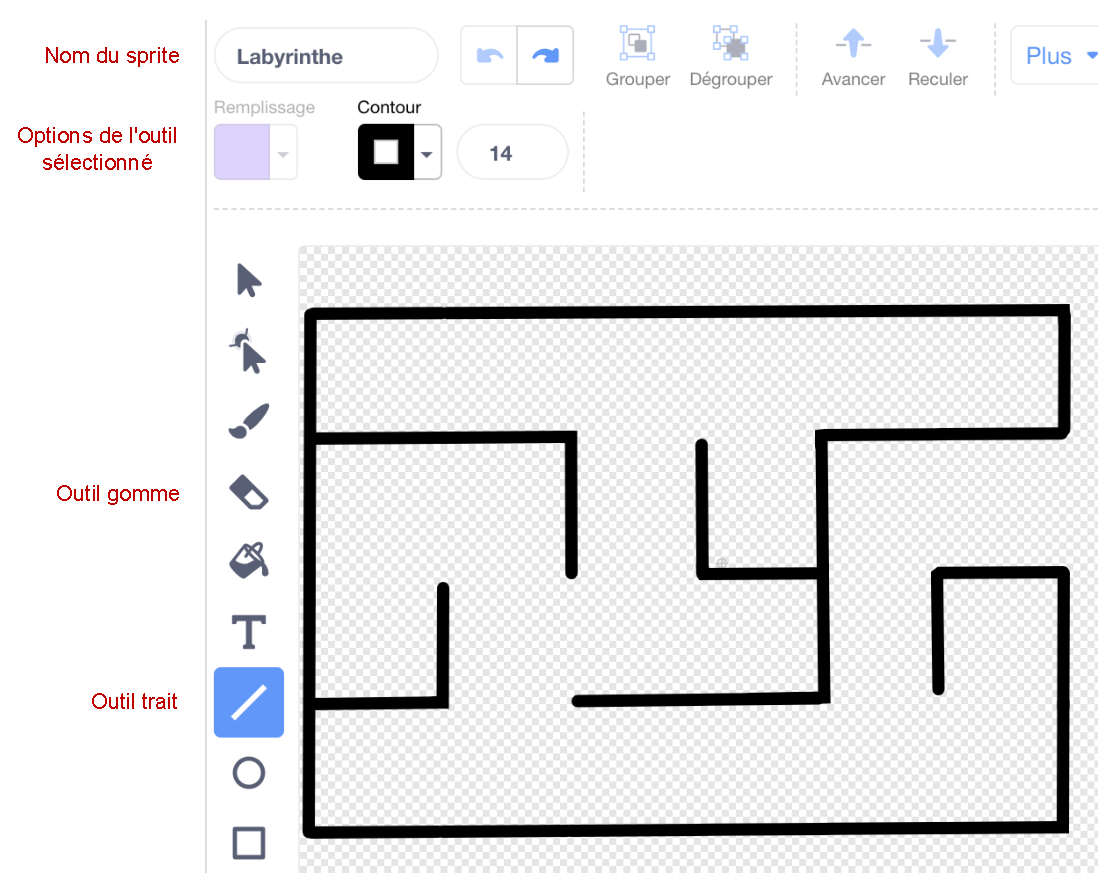
\includegraphics[width=8cm]{Scratch_labyrinthe}
            \end{minipage}
            \qquad
            \begin{minipage}{6cm}
               Créer un labyrinthe : pour cela cliquer sur \textcolor{B1}{Choisir un sprite} et sélectionner \textcolor{B1}{Peindre}. L'onglet \textcolor{B1}{Costumes} s'ouvre avec une fenêtre permettant de dessiner. \\
               Les outils principaux à utiliser pour dessiner le labyrinthe sont le \textcolor{B1}{trait} et la \textcolor{B1}{gomme}. \\
               Il est possible de configurer l'épaisseur du trait et sa couleur dans les options. \\
               Renommer le dessin sous le nom de \og Labyrinthe \fg.
            \end{minipage}
      \end{enumerate}
   
   \partie[placer et déplacer]
      \begin{enumerate}
      \setcounter{enumi}{3}
         \item {\bf Placement du chasseur et de la proie dans le labyrinthe} \pfh{} \\
         En utilisant la souris, placer le chasseur sur le point de départ du labyrinthe et placer la proie dans le labyrinthe \parbox{2.5cm}{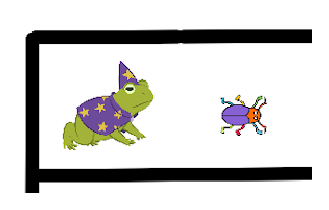
\includegraphics[width=2.5cm]{Scratch_lutins_taille}} Adapter leur \textcolor{B1}{taille} dans la fenêtre en bas à droite : \parbox{3cm}{
\includegraphics[width=3cm]{Scratch_taille}} \\ \medskip
   
         \item {\bf Programmation des flèches de déplacement} \pfh{} \\
      Pour déplacer le chasseur, il faut définir un programme pour chacune des quatre flèches de direction du clavier. \\
      Cliquer sur le lutin {\it Chasseur} puis créer ces quatre programmes dans la fenêtre de script de ce lutin. \\
         \begin{center}
            \begin{scratch}
                 \blockinitclone{quand la touche \selectmenu{flèche haut} est pressée}
               \blockmove{s'orienter à \ovalnum{0}}
               \blockmove{avancer de \ovalnum{10} pas}
            \end{scratch}
   
            \begin{minipage}{7cm}
               \begin{scratch}
                  \blockinitclone{quand la touche \selectmenu{flèche gauche} est pressée}
                  \blockmove{s'orienter à \ovalnum{-90}}
                  \blockmove{avancer de \ovalnum{10} pas}
               \end{scratch}
            \end{minipage}
            \hfill
            \begin{minipage}{7cm}
               \begin{scratch}
                  \blockinitclone{quand la touche \selectmenu{flèche droite} est pressée}
                  \blockmove{fixer le sens de rotation \selectmenu{gauche-droite}}
                  \blockmove{s'orienter à \ovalnum{90}}
                    \blockmove{avancer de \ovalnum{10} pas}
               \end{scratch}
            \end{minipage}
   
            \begin{scratch}
               \blockinitclone{quand la touche \selectmenu{flèche bas} est pressée}
               \blockmove{s'orienter à \ovalnum{180}}
               \blockmove{avancer de \ovalnum{10} pas}
            \end{scratch}
         \end{center} \medskip
         Vérifier que ces programmes fonctionnent en déplaçant le chasseur.
   
\pagebreak

         \item {\bf Création des contraintes du labyrinthe} \pfh{} \\
         \begin{minipage}{9cm}
            Le chasseur ne doit pas pouvoir traverser les murs du labyrinthe, il faut donc créer un programme qui fait \og rebondir \fg{} le chasseur lorsqu'il percute un mur. \\
            Créer ce programme pour le lutin chasseur. \\
            Dans le programme, on remarque la présence du block \textcolor{B1}{aller à} qui indique les cordonnées du chasseur déjà placé sur l'écran. Cela permet de réinitialiser sa position à chaque début de partie. \\
         \end{minipage}
         \qquad
         \begin{minipage}{6cm}
            \begin{scratch}
               \blockinitclone{quand \greenflag est cliqué}
               \blockmove{aller à x : \ovalnum{-157} y : \ovalnum{133}}
               \blockinfloop{répéter indéfiniment}
                  {\blockif{si \boolsensing{touche le \ovalsensing{Labyrinthe} ?} alors}
                     {\blockmove{tourner \turnright{} de \ovalnum{90} degrés}
                     \blockmove{avancer de \ovalnum{10} pas}
                     }
                  }
            \end{scratch}
         \end{minipage}
      \end{enumerate}
   
   \partie[créer et programmer le compteur]
      \begin{enumerate}
      \setcounter{enumi}{6}
         \item {\bf Création du compteur} \pfh{} \\
            \hspace*{0.5cm}
            \begin{minipage}{4.5cm}
               {\blue 
\includegraphics[width=3.3cm]{Scratch_compteur}} \medskip
            \end{minipage}
            \qquad
            \begin{minipage}{10cm}
               Le chasseur va aller manger une à une les proies, un compteur doit indiquer le nombre de proies restantes tout au long du jeu. Nous allons donc créer une variable qui dénombre les proies restant en jeu. \\
               Trouver le bloc \textcolor{B1}{Créer une variable} puis y donner un nom, par exemple {\it Nombre de proies restantes}.
            \end{minipage}

         \item {\bf Programmation du compteur et de la disparition des proies} \pfh{} \\
            \begin{minipage}{9cm}
               Lorsque le chasseur arrive sur sa proie, il la mange, celle-ci disparaît et le compteur est réduit de 1. \\
               Faire le programme suivant pour le lutin \textcolor{B1}{Proie}. \\
               On peut ajuster le compteur sur l'écran en le plaçant à un endroit où il ne gène pas le jeu.
            \end{minipage}
            \qquad
            \begin{minipage}{7cm}
               \begin{scratch}
                  \blockinitclone{quand \greenflag est cliqué}
                  \blockvariable{mettre \selectmenu{Nombre de cafards restants} à \ovalnum{5}}
                  \blocklook{montrer}
                  \blockinfloop{répéter indéfiniment}
                     {\blockif{si \boolsensing{touche le \ovalsensing{Grenouille} ?} alors}
                        {\blockvariable{ajouter \ovalnum{-1} à  \selectmenu{Nombre de cafards restants}}
                        \blocksound{jouer le son \selectmenu{pop} jusqu'au bout}
                        \blocklook{cacher}
                        }
                     }
               \end{scratch}
            \end{minipage}
    
         \item {\bf Ajout des autres proies} \pfh{} \\
            Nous avons fixé les proies à cinq, il faut donc les ajouter. Pour cela, il suffit de sélectionner la proie déjà créée et de la \textcolor{B1}{dupliquer} autant de fois que nécéssaire. Un clic droit sur le lutin proie permet de faire cela rapidement. \\
            Placer alors les quatre autres proies dans le labyrinthe.
      \end{enumerate}   
    
   \partie[let's go !]
      Placer le jeu en plein écran grâce au pictogramme \parbox{1cm}{
\includegraphics[width=0.7cm]{Scratch_plein_ecran}}, appuyer sur le {\textcolor{B1}{drapeau vert}} et jouer !!!
